\documentclass[11pt]{article}
\usepackage{hyperref}
\usepackage{graphicx}
\usepackage{float}
\usepackage{geometry}

\geometry{
a4paper,
total={170mm,257mm},
left=20mm,
top=20mm,
}
\hypersetup{
    colorlinks=true,
    linkcolor=blue,
    filecolor=magenta,      
    urlcolor=cyan,
}

\title{Analyzing Patterns of Computational Similarity between Kinase Ligands}
\author{Jack Ringer}
\date{July 2025}


\begin{document}

\maketitle


\section*{Abstract}
Protein kinases are relevant to a large number of human pathologies, including cancer, immune disorders, and infectious diseases. An improved understanding of structure-activity relationships for kinase ligands would benefit the development of new treatments for these pathologies. The entire workflow developed as part of this project can be found on GitHub: \href{https://github.com/Jack-42/ligandActivityAnalysis}{https://github.com/Jack-42/ligandActivityAnalysis}.


\section*{Introduction and Background}

\begin{figure}[H]
    \centering
    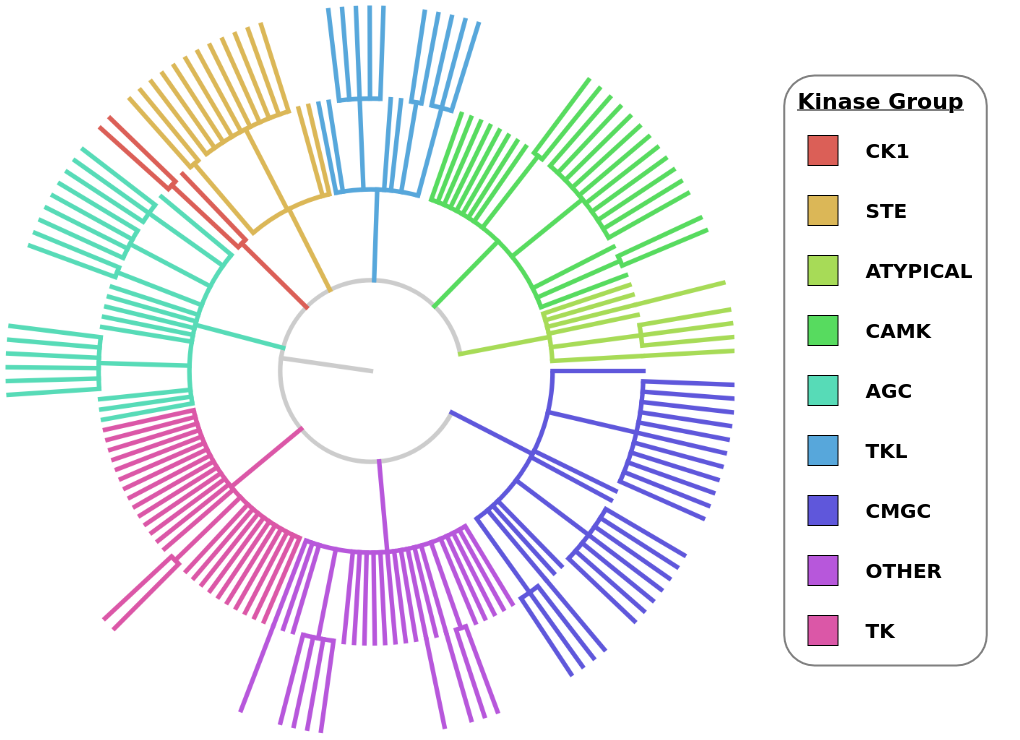
\includegraphics[width=0.7\textwidth]{../figures/protein_family_tree.png}
    \caption{Phylogenetic Tree of the Human Kinome showing major groups as well as families and subfamilies. Generated using ETE4 with data from CheMBL.}
    \label{fam_tree}
\end{figure}


\section*{Methodology}

\section*{Results}
\subsection*{Distribution}

Figure~\ref{violin_plot} provides distributions for the ${N\choose 2}$ similarity values per group ($N$ = number of ligands), as well as the ${9,995 \choose 2} = 49,945,015$ similarity values calcualted for all kinase ligands in the dataset. Table~\ref{results_table} provides additional statistics for each group, as well as results from a Mann-Whitney U test (MWUT).
\begin{figure}
    \centering
    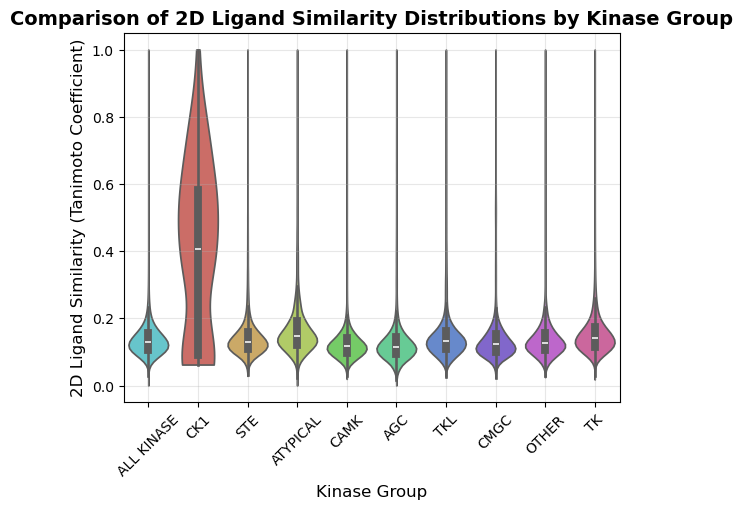
\includegraphics[width=0.75\textwidth]{../figures/violin_plot.png}
    \caption{Comparison of 2D structural similarity distributions by kinase group}
    \label{violin_plot}
\end{figure}

\begin{table}[!ht]
\centering
\resizebox{\textwidth}{!}{\begin{tabular}{|l|l|l|l|l|l|}
    \hline
    \textbf{Kinase Group} & \textbf{N. Targets} & \textbf{N. Ligands} & \textbf{Group Median} &\textbf{Comparison Median} & \textbf{MWUT p-value} \\ \hline
    CK1 & 10 & 13 & 0.407 & 0.129 & $3.10 \times 10^{-11}$ \\ \hline
    STE & 45 & 425 & 0.131 & 0.129 & $2.48 \times 10^{-169}$ \\ \hline
    ATYPICAL & 15 & 357 & 0.149 & 0.129 & $< 5 \times 10^{-324}$ \\ \hline
    CAMK & 65 & 597 & 0.117 & 0.130 & $1.0$ \\ \hline
    AGC & 59 & 809 & 0.116 & 0.131 & $1.0$ \\ \hline
    TKL & 37 & 810 & 0.133 & 0.129 & $< 5 \times 10^{-324}$ \\ \hline
    CMGC & 58 & 1275 & 0.122 & 0.130 & $1.0$ \\ \hline
    OTHER & 56 & 727 & 0.127 & 0.129 & $1.0$ \\ \hline
    TK & 80 & 5347 & 0.140 & 0.121 & $< 5 \times 10^{-324}$ \\ \hline
\end{tabular}}
\caption{Table showing comparisons of targets, ligands, and ligand similarity distributions per kinase group. Shown p-values are calculated (with Bonferroni correction) from a MWUT where the alternative hypothesis is that the similarity values within the group are stochastically greater than the distribution of all similarity values.}\label{results_table}
\end{table}



\subsection*{Enrichment}

\section*{Discussion}
% include limitations here

\section*{Conclusion}


\section*{Acknowledgement}
Much thanks to my advisor Dr.~Vincent Metzger for his guidance and input over the course of this project. I'd also like to thank Dr.~Jeremy Yang, Dr.~Cristian Bologa, and Dr.~Praveen Kumar for their feedback during weekly meetings over the course of the internship. Finally, I'd like to thank the   authors of ChEMBL DB~\cite{chembl_db_2023}.

\bibliographystyle{plain}\bibliography{report}

\end{document}
